\begin{figure}
    \centering
    \begin{subfigure}{0.41\linewidth}
        \includegraphics[width=\linewidth]{images/finetuning/simplenet_mnist_finetuning_per_arch_1e-05.eps}
        \caption{SimpleNet, fine-tuned with $\alpha=10^{-5}$}
        \label{fig:finetuning-smalllr-allmethods-perarch-simplenet_mnist}
    \end{subfigure}
    \quad
    \begin{subfigure}{0.41\linewidth}
        \includegraphics[width=\linewidth]{images/finetuning/simplenet_mnist_finetuning_per_arch_001.eps}
        \caption{SimpleNet, fine-tuned with $\alpha=10^{-2}$}
        \label{fig:finetuning-largelr-allmethods-perarch-simplenet_mnist}
    \end{subfigure}
    \quad
    \begin{subfigure}{0.41\linewidth}
        \includegraphics[width=\linewidth]{images/finetuning/lenet1_finetuning_per_arch_1e-05.eps}
        \caption{LeNet-1, fine-tuned with $\alpha=10^{-5}$}
        \label{fig:finetuning-smalllr-allmethods-perarch-lenet1}
    \end{subfigure}
    \quad
    \begin{subfigure}{0.41\linewidth}
        \includegraphics[width=\linewidth]{images/finetuning/lenet1_finetuning_per_arch_001.eps}
        \caption{LeNet-1, fine-tuned with $\alpha=10^{-2}$}
        \label{fig:finetuning-largelr-allmethods-perarch-lenet1}
    \end{subfigure}
    \quad
    \begin{subfigure}{0.41\linewidth}
        \includegraphics[width=\linewidth]{images/finetuning/lenet3_finetuning_per_arch_1e-05.eps}
        \caption{LeNet-3, fine-tuned with $\alpha=10^{-5}$}
        \label{fig:finetuning-smalllr-allmethods-perarch-lenet3}
    \end{subfigure}
    \quad
    \begin{subfigure}{0.41\linewidth}
        \includegraphics[width=\linewidth]{images/finetuning/lenet3_finetuning_per_arch_001.eps}
        \caption{LeNet-3, fine-tuned with $\alpha=10^{-2}$}
        \label{fig:finetuning-largelr-allmethods-perarch-lenet3}
    \end{subfigure}
    \quad
    \begin{subfigure}{0.41\linewidth}
        \includegraphics[width=\linewidth]{images/finetuning/lenet5_finetuning_per_arch_1e-05.eps}
        \caption{LeNet-5, fine-tuned with $\alpha=10^{-5}$}
        \label{fig:finetuning-smalllr-allmethods-perarch-lenet5}
    \end{subfigure}
    \quad
    \begin{subfigure}{0.41\linewidth}
        \includegraphics[width=\linewidth]{images/finetuning/lenet5_finetuning_per_arch_001.eps}
        \caption{LeNet-5, fine-tuned with $\alpha=10^{-2}$}
        \label{fig:finetuning-largelr-allmethods-perarch-lenet5}
    \end{subfigure}
    
    \begin{subfigure}{\linewidth}
    \centering
    \includegraphics[height=1cm]{images/finetuning/legend_finetuning_per_arch_colors.eps}
    %\quad
    %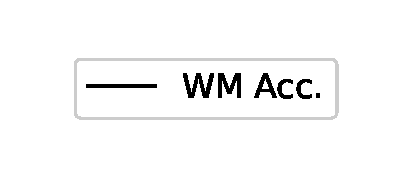
\includegraphics[height=1cm]{images/finetuning/legend_finetuning_per_arch_linestyles.eps}
    \end{subfigure}
    
    \caption{Influence of the trigger set size on robustness against fine-tuning on MNIST models. Each plot on the left corresponds fine-tuning with a small learning rate and each plot on the right to fine-tuning with a large learning rate, all of them show the results for all watermarking methods.}
    \label{fig:finetuning-mnistmodels-perarch}
\end{figure}
% The black dash-dotted line corresponds to the benchmark test accuracy of the non-watermarked model.